\documentclass{article}

%packages included
\usepackage{amsmath}
\usepackage{graphicx}
\usepackage{tabularx}		% lets you choose width of tabular(x) environment
\usepackage{hyperref}
\hypersetup{
    colorlinks=true,
    linkcolor=black,
    filecolor=magenta,
    urlcolor=cyan,
    pdftitle={RoadAI project plan},
    }
%\usepackage{titlesec}		% see redefinition of \section command
%\uepackagr{minted}		% compile with -shell-escape flag to get syntax highlighting for code blocks (\begin{minted}{<programming lang>} <...>\end{minted}, \inputminted{programming lang}{filename})
%\usepackage{times}		% Times New Roman. \documentclass{article}[12] gives 12 pt. writing.
\usepackage{hyperref}

%custom commands:
\newcommand{\vectorarrow}{\overset{\rightharpoonup}}
%\titleformat{\section}{\normalfont\Large\bfseries}{\thesection}{1em}{}[\hrule]		% redefines \section command. if active along with package "titlesec", will add line under title of each new section
\makeatletter
\renewcommand\@makefntext[1]{\leftskip=2em\hskip-2em\@makefnmark#1}
\makeatother

\title{Project Plan - RoadAI}
\author{Berezin, Ilya; Hasle, Viktor R.; Hatland, Ada; Ringkjoeb, Elias}
\date{September $6^{th}$ 2023}
%Setting line spacing
\renewcommand{\baselinestretch}{1.5}

\begin{document}

% \begin{titlepage}
\maketitle
% \tableofcontents
% \end{titlepage}

%---------------------------------
\section{Overall goal}
In the RoadAI project, we plan to use Multi Agent Reinforcement Learning to reduce emissions coming from
construction machines. Using a data set provided from NORA (Norwegian Artificial Research Consortium) consisting of GPS, vibration and drone data, the goal is to reduce the overall emissions from road construction. We intend to utilize MARL as a techninque to optimize
the trucks idle time as they haul construction materials.

%---------------------------------
\section{Step-by-step plan}
\begin{enumerate}
  \item Read up on general MARL.
  \item Propose a high-level design idea.
  \item Make a directory structure for the code, and commit to GitHub.
  \item Create environment for MARL in pettingzoo.
  \item Implement algorithm for MARL. 
  \item Tune hyperparameters
  \item Evaluate performance of the algorithm.
\end{enumerate}

%---------------------------------
\section{Meeting plan}
We will be having inperson weekly meetings to discuss our progress. Depending on the workflow we may decide to 
meet more frequently. In addition, we will be meeting with our supervisor for this project biweekly. This way,
we will be able to communicate effectively and often. We have also set up a discord channel where we are able to more quickly collaborate.

%---------------------------------
\section{Methods/tools}
There are several \texttt{python} libraries which will be useful for us in this project.
Among these libraries are the following:
\begin{description}
  \item[PettingZoo] We will be using PettingZoo\footnote[1]{\url{https://pettingzoo.farama.org}}
    to create the environments for the MARL system.
  \item[Rllib] We will be using Rllib\footnote[2]{\url{https://docs.ray.io/en/latest/rllib/index.html}}
    for agent implentation.
  \item[PyMARL] PyMARL\footnote[3]{https://github.com/oxwhirl/pymarl} is a PyTorch based library
    developed for MARL problems specifically. The library was made specificaly to solve the StarCraft
    Multi-Agent Challenge (SMAC)\footnote[4]{Samvelyan, M., Rashid, T., De Witt, C. S., Farquhar, G., Nardelli, N., Rudner, T. G., ... \& Whiteson, S. (2019). The starcraft multi-agent challenge. \textit{arXiv preprint arXiv:1902.04043}.}. %APA formatting
    This library features implementations of baseline as well as state-of-the-art algorithms.
\end{description}

%----
\noindent
Various research articles studying MARL problems have utilized algorithms which have potential for our
project.

\noindent
In additoin to the aforementioned tools, there is a chance that we may discover some other libraries and/org
algorithms which work better for out project. In such a case, we might consider using these.

\noindent
Lastly, the University of Oslo offers computational resources, which we might consider using in order to
train our model in a faster fashion, as RL training can be quite demanding. Also parts of the data we will be using is quite extensive.

%---------------------------------
\section{Timeline}
\begin{figure}[h]
    \begin{center}
        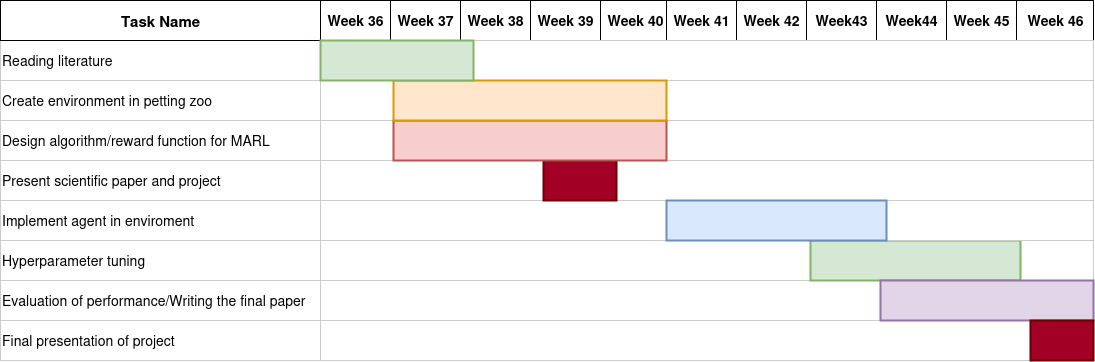
\includegraphics[width=\textwidth]{Timeline.png}
    \end{center}
    \caption{Timeline}
    \label{fig:timeline}
\end{figure}

%---------------------------------
\section{Responsibilities overview}
 We have chosen to divide the project responsibilities into two main parts: environment creation
 and implementation and testing of algortithms. The thought is for all of us to be able to cooperate on both parts, but we will divide
 the responsibilities such that Ada and Viktor has the main responsibility for enviroment creation, and Elias and Ilya has the main responsibility for implementing and testing algorithms.
\\
Later in the project we will all work together to combine what we have worked on to a complete system. 
We will also intend to share the responsibility of evaluting/tuning our system as discussion really
facilitates that. 


%---------------------------------
% \section*{References}
% \begin{enumerate}
%   \item https://pettingzoo.farama.org
%   \item https://docs.ray.io/en/latest/rllib/index.html
% \end{enumerate}

\end{document}
